\documentclass[UROP.tex]{subfiles}
\begin{document}

\bigskip
\section{\Large Background}
	Phased array systems are typically used in scenarios in which the antenna's beam must be rotated very quickly or the antenna must be mounted to a jostling structure that endangers the mechanical integrity of the antenna.  Phased arrays can be used for radar, communication, or imaging.   \\
	
	Phased array systems have been designed for many use cases at operating frequencies that depend on the application.  A phased array allows for fast steering of a very directed beam.  Higher frequency phased arrays have been used for this application, however these phased arrays have limited range due to increased free space attenuation at high frequencies.  This phased array system shall work at 900 MHz, which allows for communication at distances up to 20 miles.  In order to establish a long range link, we propose a 3D array to obtain higher gain at lower elevation angles. \\
	
	Members in our group are well educated in antenna design: some members have worked in RF research labs and others at RF companies.  
	
\begin{figure}[H]
\centering
	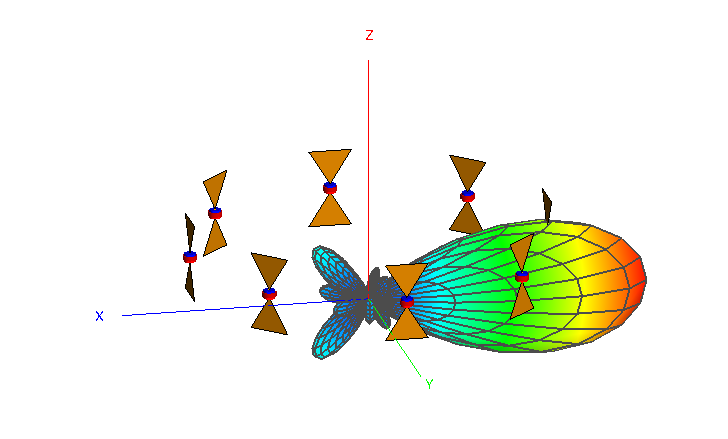
\includegraphics[scale=0.5]{PhasedArrayExample.png}
	\caption{ Phased Array example showing the ability to steer a beam\label{fig:PAexample}}
\end{figure}
	
	As seen in Fig.~\ref{fig:PAexample}, the ability to steer a beam is inherent in the design of a phased array.  By changing the phases in which the antenna elements are fed, the beam can be steered in any direction. This array is a preliminary design to the 3D array that will be the final product.  Some of the students in this group worked with phased array systems and will use that experience to design a better, longer range phased array system.  
\end{document}
